\subsection{EU Nuclear Operation until 2050}

\begin{frame}
	\frametitle{Historical Operation of EU Reactors}

\begin{table}[h]
	\centering
	\scalebox{0.86}{
		\begin{tabular}{cccc}
			\hline
			\textbf{Category } & \textbf{Value} & \textbf{Unit} & \textbf{Specifics}\\ \hline
			Total UOX Usage  & 164,014 & MTHM &  \\ 
			Total MOX Usage  & 6,372 & MTHM & \\ 
			Total Used UOX Stored  & 111,565 & MTHM & \gls{UNF} that is not reprocessed\\  
			Total Used UOX Stored (France) & 18,564 & MTHM & \gls{UNF} that is not reprocessed \\
			Total Tailings  & 986,603 & MTHM & \\ 
			Total Natural U Used  & 1,157,145 & MTHM & \\ \hline
		\end{tabular}}
		\caption{Simulation Results for Historical Nuclear Operation 
		of \gls{EU} Nations}
		\label{tab:sim_result}
\end {table}

\end{frame}

\begin{frame}
	\frametitle{Tails and UNF Inventory}
\begin{figure}[htbp!]
\begin{minipage}[b]{.45\linewidth}
	\begin{center}
		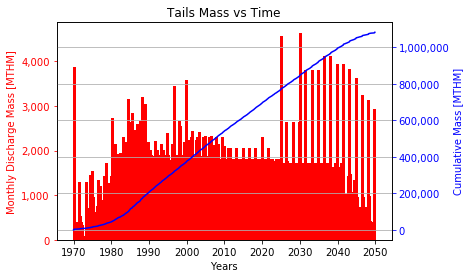
\includegraphics[width=\textwidth]{./images/eu_future/tails.png}
	\end{center}
	\caption{Timeseries of Tails Mass in the \gls{EU}.}
	\label{fig:eu_tail}
\end{minipage}
\hspace{.5cm}
\begin{minipage}[b]{.45\linewidth}
	\centering
	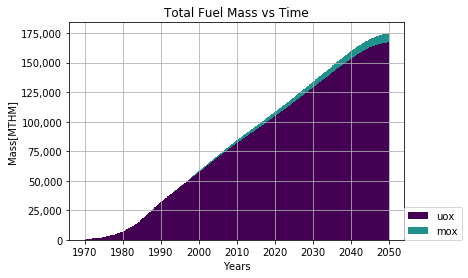
\includegraphics[width=\textwidth]{./images/eu_future/total_fuel.png}
	\caption{Timeseries of Total Fuel Usage in \gls{EU}.}
	\label{fig:eu_fuel}
\end{minipage}
\end{figure}
\end{frame}

\begin{frame}

\begin{figure}[htbp!]
	\begin{center}
			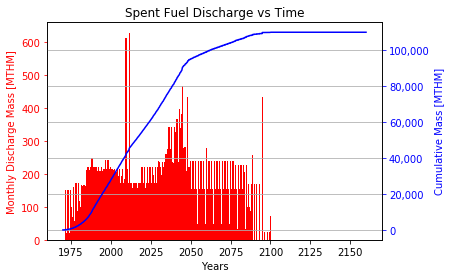
\includegraphics[scale=0.7]{./images/eu_future/snf_discharge.png}
	\end{center}
	\caption{Timeseries of Used Nuclear Fuel in \gls{EU}.}
	\label{fig:eu_snf}
\end{figure}

\end{frame}

\begin{frame}
	\frametitle{Plutonium in Legacy UNF}
	
\begin{table}[h]
	\centering
	\begin{tabular}{ccc}
		\hline
		\textbf{Isotope} & \textbf{Mass Fraction in Used Fuel [\%]} & \textbf{Quantity [t]} \\ \hline
		Total & 0.9358 & 1,044 \\ 
		Pu238 & 0.0111 & 12.3 \\ 
		Pu239 & 0.518 & 577.9 \\ 
		Pu240 & 0.232 & 258.8 \\ 
		Pu241 & 0.126 & 140.5 \\ 
		Pu242 & 0.0487 & 54.3 \\ \hline
	\end{tabular}
	\caption{Plutonium From Used Fuel}
	\label{tab:pu}
\end{table}
\end{frame}


\subsection{French Transition Scenario ~2160}

\begin{frame}
	\frametitle{SFR Deployment with Legacy UNF}
	\begin{itemize}
		\item Reprocessing UNF from all EU nations can start approx. 213 SFRs.
		\item Two generations of 66GWe SFRs = 220 SFRs
		\item Breeding Ratio of SFRs over one. ($\frac{23.95}{22.0} = 1.088$)
		\item Initial Pu loading of $4.9$ tons for ASTRID-type SFR \cite{varaine_pre-conceptual_2012}.
		\item $\frac{Pu \ from \ legacy \ \gls{UNF}}{4.9} \approx 213$
	\end{itemize}
\end{frame}

\begin{frame}
	\frametitle{Frech Transition Results}
	
\begin{table}[h]
	\centering
	\scalebox{0.86}{
		\begin{tabular}{ccc}
			\hline
			\textbf{Category} & \textbf{Unit} & \textbf{Value}  \\ \hline
			Total MOX used & MTHM & 63,820  \\ 
			Total \glspl{SFR} Deployed & & 220 \\ 
			Total Plutonium Reprocessed & MTHM & 17,303 \\ 
			Total MOX from UOX Waste & MTHM & 3,056  \\ 
			Total MOX from MOX Waste & MTHM  & 60,763 \\ 
			Total Tails used & MTHM & 58,076 \\ 
			Total legacy UNF reprocessed & MTHM & 71,726 \\ 
			Total Reprocessed Uranium Stockpile & MTHM & 150,098 \\ 
			Total Raffinate & MTHM & 17,303 \\ \hline
		\end{tabular}}
		\caption {\gls{SFR} Simulation Results}
		\label{tab:sfr_sim_result}
\end {table}


\end{frame}

\begin{frame}
	\frametitle{Material Flow in French Transition Scenario}
	
\begin{figure}[htbp!]
\begin{minipage}[b]{.45\linewidth}
	\begin{center}
		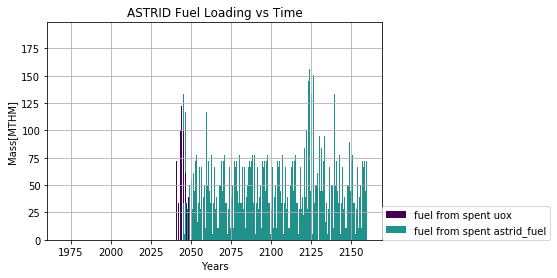
\includegraphics[width=\textwidth]{./images/french-transition/where_fuel.png}
	\end{center}
	\caption{Timeseries of fuel loaded into \glspl{SFR}}
	\label{fig:fuel}
\end{minipage}
\hspace{.5cm}
\begin{minipage}[b]{.45\linewidth}
	\centering
		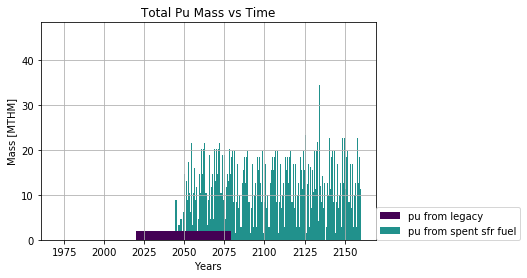
\includegraphics[width=\linewidth]{./images/french-transition/pu.png}
	\caption{Separated plutonium discharge from Reprocessing Plant}
	\label{fig:pu_no_cum}
\end{minipage}
\end{figure}

\end{frame}